\section{Experiments}\label{sect_exp}
% Give results of experiments.
% It is also necessary to compare the performance with FTRL.

In this chapter
we give results of experiments on the number of resampling of geometric resampling
and compare the regret and computational efficiency with existing algorithms.
All of the figures are the results of $100$ trials. The experiments were conducted on an AMD EPYC 7763 CPU, implemented in Python~3.9 using the NumPy library. 
The code is available at: \url{https://github.com/BotaoChen123/FTPL-CGR}\footnote{Adapted from the code of \citet{pmlr-v206-tsuchiya23a} available at \url{https://github.com/tsuchhiii/bobw-variance/tree/master}.}.

%we first compare the number of resampling of
%the FTPL with conditional geometric resampling ({\sf{FTPL~CGR~I}}, FTPL~CGR~II-unbiased, FTPL~CGR~II-biased) with FTPL with geometric resampling ({\sf{FTPL~GR}}).
%We then compare the regret and computational efficiency between these FTPLs and Tsallis-INF, that is, FTRL with Tsallis-entropy regularizer.

\paragraph{Environments}
Following \citet{JMLR:v22:19-753}, we consider
the stochastically constrained adversarial setting
and
the stochastic setting,
% The details of the instances as well as the additional results are given in Appendix~\ref{append_sup_exp}.
where the losses of each arms follow the Bernoulli distributions, and we exclusively consider the case where the suboptimality gap $\Delta=0.125$. For the stochastic setting, which is implemented for the experiments shown in Appendix~\ref{append_sup_exp}, the mean losses are decided as $\qty(1-\Delta)/2$ for the single optimal arm and $\qty(1+\Delta)/2$ for the other suboptimal arms.

\begin{figure}[h]
    \begin{minipage}[c]{0.48\textwidth}
        \centering
        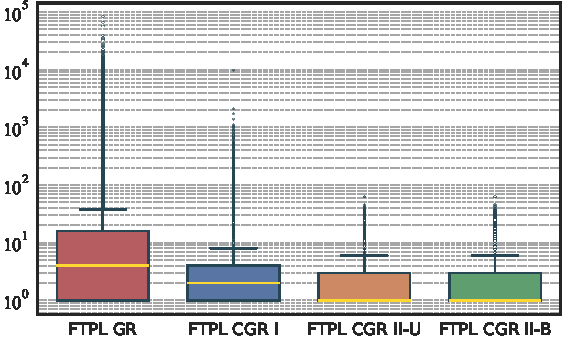
\includegraphics[width=\textwidth, height=0.6\textwidth]{figures/boxplot_smallfig/box_32_adv.pdf}
        \captionsetup{justification=centering} 
\vspace{-6mm}
        \caption{Number of resampling for adversarial setting and $K=32$.}
        \label{fig:box_32_adv}
    \end{minipage}\quad
    \begin{minipage}[c]{0.48\textwidth}
        \centering
        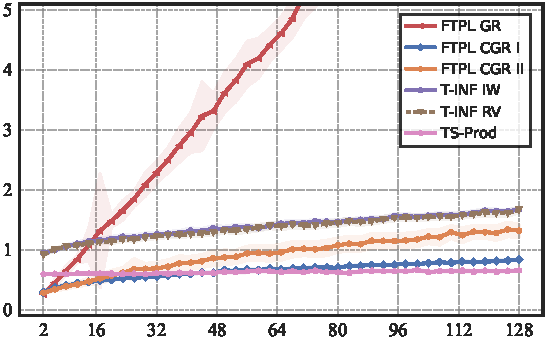
\includegraphics[width=\textwidth, height=0.6\textwidth]{figures/runtime_adv_5.pdf} 
\vspace{-6mm}
        \caption{Runtime (sec) for adversarial setting and different $K$.}
        \label{fig:runtime_adv}
    \end{minipage}

\vspace{5mm}
   \begin{minipage}[b]{\textwidth}
            \centering
            \begin{subfigure}[c]{0.4\textwidth}
                \centering
                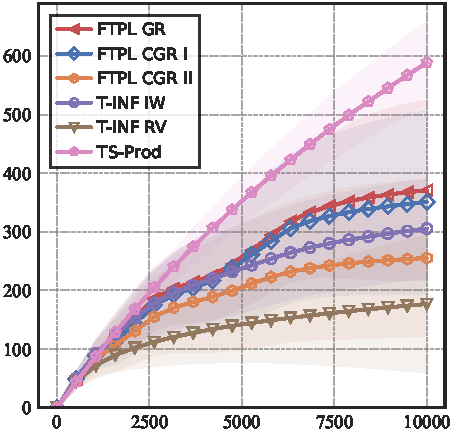
\includegraphics[width=0.98\textwidth]{figures/regret_smallfig/s_6_na_8_d_8_dist_SCA-Ber_m_mab_nv_1.0.pdf}
\vspace{-1mm}
                \caption{$K=8$}
                \label{fig:regret_8_adv}
            \end{subfigure}\qquad\qquad\quad
            \begin{subfigure}[c]{0.4\textwidth}
                \centering
                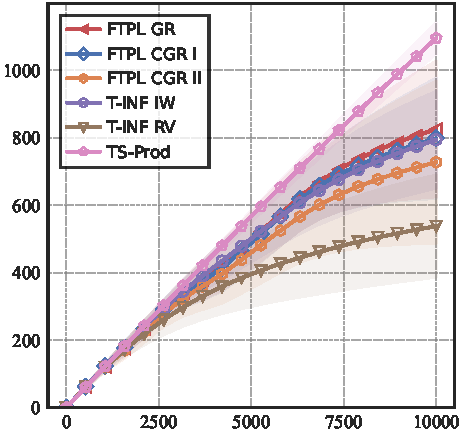
\includegraphics[width=0.98\textwidth]{figures/regret_smallfig/s_6_na_32_d_32_dist_SCA-Ber_m_mab_nv_1.0.pdf}
\vspace{-1mm}
                \caption{$K=32$}
                \label{fig:regret_32_adv}
            \end{subfigure}
            % \nextfloat
\vspace{-2mm}
            \caption{Pseudo regret in adversarial setting.}
            \label{fig:regret_adv}
    \end{minipage}
    \vspace{-1.5em}
\end{figure}

For the stochastically constrained adversarial setting, which is implemented for the experiments shown in 
% Figures~\ref{fig:box_32_adv}, \ref{fig:runtime_adv}, \ref{fig:regret_adv}, \ref{fig:scatter_mean_32_adv} and \ref{fig:scatter_max_32_adv}, 
Figures~\ref{fig:box_32_adv}--\ref{fig:regret_adv},
the mean losses for the single optimal arm and the suboptimal arms switch between $\qty(1-\Delta, 1)$ and $\qty(0, \Delta)$, with the duration of each phase growing exponentially by a factor of $1.6$ after every switch. Both settings are similar to those in \citet{JMLR:v22:19-753}. 
Since we observed the same tendency between both settings,
we only give the results for the former setting, and the results for the stochastic setting as well as the additional results are given in the appendix.

%\honda{I recommend to use a different font for algorithm names like \sf{FTPL CGR I}}.
\paragraph{Algorithms}
We compare FTPL with three variants of conditional geometric resampling
(CGR~I, CGR~II-unbiased, CGR~II-biased) with FTPL with geometric resampling,
which we will respectively write
\CGRI, \CGRIIU, \CGRIIB, and \GR.
%FTPL~CGR~I, FTPL~CGR~II-unbiased, FTPL~CGR~II-biased,  {\sf{FTPL~GR}}
In all the experiments we used Fr\'{e}chet distribution with shape $\alpha = 2$ for the perturbation of {\sf{FTPL}}.

%We compare three variants of FTPL with conditional geometric resampling({\sf{FTPL~CGR~I}}, FTPL~CGR~II-unbiased, FTPL~CGR~II-biased) with FTPL with geometric resampling ({\sf{FTPL~GR}}).
%% in terms of the number of generated samples at every round.
%For convenience, we write CGR~II-unbiased and CGR~II-biased as {\sf{CGR~II-U}} and {\sf{CGR~II-B}} in the figure.
%For all the experiments in our paper, the perturbation in {\sf{FTPL}} follows Fr\'{e}chet distribution with shape $\alpha = 2$.



We also compare the performance with {\sf{Tsallis-INF}} and {\sf{TS-Prod}}. 
{\sf{Tsallis-INF}} is {\sf{FTRL}} with Tsallis-entropy regularizer. 
In our experiments, $w_t$ in this policy is computed by Newton's method. 
For the loss estimator of Tsallis-INF,
we consider Importance-Weighted (IW) estimator and Reduced-Variance estimator (RV, \citealp{JMLR:v22:19-753}), the latter of
which has better regret bounds than the former.
We denote Tsallis-INF with these estimators respectively as {\sf{T-INF~IW}} and {\sf{T-INF~RV}}.

We used the same learning rate for {\sf{T-INF}} as that of \citet{JMLR:v22:19-753}
($\eta_t=c/\sqrt{t}$ with $c=2$ for IW and $c=4$ for RV).
Since FTPL in this thesis and those in \citet{pmlr-v247-lee24a, pmlr-v201-honda23a} are designed to mimic {\sf{T-INF~IW}},
we use the same learning rate for {\sf{FTPL}} as that of {\sf{T-INF~IW}}.

{\sf{TS-Prod}} is a variant of Prod \citep{cesa2007improved} derived from {\sf{FTRL}}, serving as an approximation of {\sf{T-INF}}. Unlike {\sf{T-INF}}, {\sf{TS-Prod}} requires only a one-step update rather than solving an optimization problem, resulting in more efficient computation with a complexity of $O(K)$. We used the same learning rate for {\sf{TS-Prod}} as that of \citet{zimmertproductive}.
%\honda{I modified the phrasing around here because Kim-Tewari tried to mimic T-INF, but not specifically for T-INF IW.}


%we consider not only IW estimator, which is also used in {\sf{FTPL}}, but also a loss estimator called Reduced-Variance estimator (RV, \citet{JMLR:v22:19-753}), which brings some improvement to regret performance. We denote Tsallis-INF with these estimators respectively as {\sf{T-INF~IW}} and {\sf{T-INF~RV}}. For all experiments in our paper, T-INF used the same learning rate as \citet{JMLR:v22:19-753} ($\eta=c/\sqrt{t}$ with $c=2$ for IW and $c=4$ for RV).  As FTPL with Fr\'{e}chet perturbation is designed to mimic {\sf{T-INF~IW}} \citep{kim2019optimality}, we also used the same learning rate for FTPL as that of {\sf{T-INF~IW}}.


\paragraph{Number of Resampling}
Figure \ref{fig:box_32_adv} shows the number of resampling at each round for adversarial setting on a log scale.
From this figure we see that the number of resampling is significantly and stably kept small under all the variants of {\sf{FTPL~CGR}}.
In particular, the medians of \CGRIIU{} and \CGRIIB{} are one, that is, resampling terminates within only one trial for more than half of the rounds.

%The box portion, along with the area below it, which together represent the lower $75\%$ of the data, reflects that, for the overwhelming majority of cases, the% number of resampling is significantly and stably reduced to a very small value under all the variants of {\sf{FTPL~CGR}}.
% As shown in Figure \ref{fig:ave_8_sto} and Figure \ref{fig:ave_32_sto},
% the average number of resampling is significantly and stably reduced under all the variants of {\sf{FTPL~CGR}}.

%Figure \ref{fig:box_32_adv} shows the number of resampling at each round for adversarial setting on a log scale
%where recall that they are results over $100$ trials.
%The box portion, along with the area below it, which together represent the lower $75\%$ of the data, reflects that, for the overwhelming majority of cases, the number of resampling is significantly and stably reduced to a very small value under all the variants of {\sf{FTPL~CGR}}.
%% As shown in Figure \ref{fig:ave_8_sto} and Figure \ref{fig:ave_32_sto},
%% the average number of resampling is significantly and stably reduced under all the variants of {\sf{FTPL~CGR}}.



% Furthermore, as can be seen from Figures~\ref{fig:max_8_sto} and \ref{fig:max_32_sto}, 
Furthermore, as observed from the outliers, the number of resampling of {\sf{FTPL~GR}} is somewhat unstable and sometimes
prohibitively large (recall that the plot is in log scale),
%becomes very large.
while {\sf{FTPL~CGR}} effectively controls the maximum number of resampling.
% particularly for large $K$.
%As $K$ becomes sufficiently large, all the variants of FTPL~CGR perform stably on the maximum times of resampling, which almost remains at a very low level.
In addition, the actual maximum number of resampling under {\sf{FTPL~CGR~II-B}}
was much smaller than the theoretical guarantee of
$G_t=(K\lor 4)\log t$, which is for example $G_t\approx 295$ for $K=32$ and $t=10000$.
For this reason the behaviors of {\sf{FTPL~CGR~II-U}} and {\sf{FTPL~CGR~II-B}} were empirically indistinguishable.
For this reason, to avoid redundancy, we present only the results for {\sf{FTPL~CGR~II-U}} in the figures of runtime and regret performance, referring to it as {\sf{FTPL~CGR~II}}.



%Figures \ref{fig:num_ave} and \ref{fig:num_max} are the results examining the behavior of FTPL~CGR and FTPL~GR, focusing on the average and maximum times of resampling per round respectively. As shown in Figure \ref{fig:num_ave}, compared with FTPL~GR, the average times of resamplings per round is effectively reduced in all the variants of FTPL~CGR.
%Furthermore, the performance of FTPL~CGR~II exceeds that of {\sf{FTPL~CGR~I}}.
%As for the maximum times of resampling, it can be observed that FTPL~GR occasionally results in a large number of resamplings, significantly increasing computational costs.
%For FTPL~CGR, the maximum times of resampling is effectively controlled, while sometimes {\sf{FTPL~CGR~I}} exhibits a slight degree of instability when $K$ is small.
%As $K$ becomes sufficiently large, all the variants of FTPL~CGR perform stably on the maximum times of resampling, which almost remains at a very low level.



\paragraph{Regret Comparison}
Figure 3 is the comparison of the regret of {\sf{FTPL}} with those of {\sf{FTPL~GR}}, {\sf{T-INF}} and {\sf{TS-Prod}}. 
As can be seen from this result, the regret of {\sf{FTPL~CGR~I}} is slightly better than {\sf{FTPL~GR}}.
Furthermore, the regret of {\sf{FTPL~CGR~II}} is close to {\sf{T-INF~IW}}, and even better in some settings,
despite the fact that {\sf{FTPL~CGR}} is also based on the IW estimator.
As discussed in Remark~\ref{remark_variance},
this improved regret of {\sf{FTPL~CGR}} seems to be thanks to the significantly reduced variance of the loss estimator.
On the other hand, the regret of {\sf{FTPL~CGR~II}} is still worse than {\sf{T-INF~RV}}.
Therefore it is still an important future work to devise a counterpart of RV estimator for FTPL.
The regret of {\sf{TS-Prod}} is the worst among all compared algorithms, seemingly due to the approximation error introduced by its update rule.


%Figure \ref{fig:regret} is the result comparing the regret performance of FTPL~CGR with that of FTPL~GR and {\sf{T-INF}}. We can see that in both settings, the behavior of {\sf{FTPL~CGR~I}} is a little better than FTPL~GR. We can also see that the behavior of both variants of FTPL~CGR~II is similar to {\sf{T-INF~IW}}, and even better than it in some settings. The improved regret performance of FTPL~CGR seems to be due to the significantly reduced variance of the loss estimator when GR is replaced with CGR.

\paragraph{Computational Efficiency}
Figure \ref{fig:runtime_adv} shows the runtime for arm selection
over $10000$ rounds
of {\sf{FTPL}}, {\sf{T-INF}} and {\sf{TS-Prod}} for varying $K$ from $2$ to $128$.
When $K$ is small enough, both of {\sf{FTPL~GR}} and {\sf{FTPL~CGR}} run much faster than {\sf{T-INF}}.
However, as $K$ increases,
the runtime of {\sf{FTPL~GR}} sharply grows,
while those of {\sf{FTPL~CGR}}, {\sf{T-INF}} and {\sf{TS-Prod}} are kept small.
In particular, the runtime of {\sf{FTPL~CGR}} and {\sf{TS-Prod}} is much smaller than {\sf{T-INF}} thanks to its optimization-free nature. Additionally, the runtime of {\sf{FTPL~CGR}} slightly exceeds {\sf{TS-Prod}} when $K$ is sufficiently large, due to the additional $\log K$ factor in its complexity.

One interesting observation is that the runtime of {\sf{FTPL~CGR~I}} is consistently better than {\sf{FTPL~CGR~II}} despite its larger number
of resampling shown in Figure~\ref{fig:box_32_adv}.
This comes from the fact that the conditioning procedure of CGR~I only needs swapping of the maximum and is very fast.



%Figure \ref{fig:runtime} is the result examining the runtime over $5000$ rounds
%of FTPL and {\sf{T-INF}} across different values of $K$, which is ranged from $2$ to $128$.
%reward-generating and the computation of the regret?
%If not, it is desirable to do that. That said, it would be not at all dominant and it has low priority.}
%When $K$ is small enough, both of FTPL~GR and FTPL~CGR run much faster than {\sf{T-INF}}. However, as $K$ grows larger, the runtime of FTPL~GR grows sharply, while the runtimes of FTPL~CGR and {\sf{T-INF}} increase at a slower rate. As a result, when $K$ becomes sufficiently large, FTPL~GR requires significantly more time compared to other algorithms. For FTPL~CGR, the runtime consistently remains better than that of {\sf{T-INF}} within the experimental range of $K$ we considered. Note that the expected times of resampling of {\sf{FTPL~CGR~I}} keeps larger than that of FTPL~CGR~II, but {\sf{FTPL~CGR~I}} runs a little faster than FTPL~CGR~II when $K$ becomes large. This result seems to be due to the fact that, when $K$ is sufficiently large, the expected number of resamplings for both algorithms remains very similar, and {\sf{FTPL~CGR~I}} has a faster sample generation speed.

